\documentclass{article}

\usepackage{color}
\usepackage{amsmath}
\usepackage{amssymb}
\usepackage{latexsym}
\usepackage{amsfonts}
%\usepackage{times}
\usepackage{url}
%\usepackage{bibspacing}
%\setlength{\bibspacing}{\baselineskip}
\usepackage{hyperref}
\usepackage{xspace}
\usepackage{graphicx}
\usepackage{listings}
\lstset{language=C++}

\renewcommand{\L}{\mathcal{L}}
\newcommand{\V}{\mathcal{V}}
\renewcommand{\P}{\mathcal{P}}
\newcommand{\poly}{\mathrm{poly}}
\newcommand{\binary}{\{0,1\}}
\newcommand{\set}[1]{\left\{#1\right\}}

\newtheorem{thm}{Theorem}[section]
\newtheorem{lem}[thm]{Lemma}
\newtheorem{cor}[thm]{Corollary}
\newtheorem{propo}[thm]{Proposition}
\newtheorem{fct}[thm]{Fact}
\newtheorem{defn}[thm]{Definition}
\newtheorem{exmp}[thm]{Example}
\newtheorem{assm}[thm]{Assumption}
\newtheorem{clm}[thm]{Claim}
\newtheorem{techclm}[thm]{Technical Claim}
\newtheorem{rem}[thm]{Remark}
\newtheorem{cons}[thm]{Construction}

\newenvironment{theorem}{\begin{thm}\begin{rm}}%
{\end{rm}\end{thm}}
\newenvironment{lemma}{\begin{lem}\begin{rm}}%
{\end{rm}\end{lem}}
\newenvironment{corollary}{\begin{cor}\begin{rm}}%
{\end{rm}\end{cor}}
\newenvironment{proposition}{\begin{propo}\begin{rm}}%
{\end{rm}\end{propo}}
\newenvironment{fact}{\begin{fct}\begin{rm}}%
{\end{rm}\end{fct}}
\newenvironment{definition}{\begin{defn}\begin{em}}%
{\end{em}\end{defn}}
\newenvironment{example}{\begin{exmp}\begin{em}}%
{\end{em}\end{exmp}}
\newenvironment{assumption}{\begin{assm}\begin{em}}%
{\end{em}\end{assm}}
\newenvironment{claim}{\begin{clm}\begin{rm}}%
{\end{rm}\end{clm}}
\newenvironment{techclaim}{\begin{techclm}\begin{rm}}%
{\end{rm}\end{techclm}}
\newenvironment{remark}{\begin{rem}\begin{em}}%
{\end{em}\end{rem}}
\newenvironment{construction}{\begin{cons}\begin{em}}%
{\end{em}\end{cons}}


\newcommand{\proref}[1]{Protocol~\protect\ref{#1}}

\newenvironment{boxfig}[2]{\begin{figure}[#1]\fbox{\begin{minipage}{\linewidth}
                        \vspace{0.2em}
                        \makebox[0.025\linewidth]{}
                        \begin{minipage}{0.95\linewidth}
            {\small{
                        #2 }}
                        \end{minipage}
                        \vspace{0.2em}
                        \end{minipage}}}{\end{figure}}


\newcommand{\pprotocol}[5]{
  {\begin{figure}[#4]
      \begin{center}
        \fbox{ \small \hbox{
            \begin{minipage}{.98\linewidth}
              \begin{center}
                \textbf{#1}
              \end{center}
              #5
            \end{minipage}
          } }
        \caption{\label{#3} #2}
      \end{center}
      \vspace{-3ex}
    \end{figure}
} }


\newcommand{\protocol}[4]{
\begin{boxfig}{htbp}{
\begin{center}
{\bf #1}
\end{center}
    #4
\vspace{0.5ex} } \caption{\label{#3} #2}
\end{boxfig}
}


\begin{document}

\section{Introduction}
In this document we explain the basic principles behind several important attacks in computer networks.  There are attacks that primarily attack the implementation and computer architecture where a protocol executes.  These attacks illuminate the importance of considering the entire environment when designing a secure protocol.  In particular, the underlying computer architecture and the code needed to implement a protocol affect the security of the protocol.  We begin by considering basic buffer overflows as well as some of the arms race that has followed in Section~\ref{sec:buffer overflows}.  Next, we consider how lose permissions in browser sandbox's allow for escalation of privileges in Section~\ref{sec:xss}.  Finally, we consider how attackers are able to compromise ``provably'' secure cryptographic algorithms by gaining extra information that outside of the model.  These are known as side-channel attacks and we review some basics in Section~\ref{sec:side channels}.

\section{Buffer Overflows}\label{sec:buffer overflows}
We review the basics of buffer overflows here so the computer architecture we present is greatly simplified.  We focus on stack-smashing techniques.  In particular, we focus our discussion on the C programming language.

When a program is executed, there are two types of variables.  Fixed-size local variables are allocated on the stack, and variables whose size is not known at compile time must be allocated through the heap.  Stack-smashing occurs because the abstraction that stack variables are fixed-size is not enforced.  We begin with the following simple example:

\begin{lstlisting}
void swap(int a, int b){
  int c =0;
  c = a;
  a=b;
  b=c;
  return;
}
\end{lstlisting}

Before this function is called the execution environment must be set up.  Let $A$ be the calling instruction.  The function $swap$ needs three values $a, b$ and what address to return to.  These are placed on the stack~(which grows down).  Finally, the program needs a local variable $c$, which is also placed on the stack.  This leads to the following state of the stack for return address $0xd0000$, $a=1$ and $b=2$:

\begin{tabular}{c|c}
$0xc020$ & $0xd000$\\
$0xc01c$ & $0x0001$\\
$0xc018$ & $0x0002$\\
$0xc014$ & $0x0000$
\end{tabular}

After the program function executes, we have an updated stack:

\begin{tabular}{c|c}
$0xc020$ & $0xd000$\\
$0xc01c$ & $0x0002$\\
$0xc018$ & $0x0001$\\
$0xc014$ & $0x0001$
\end{tabular}

Then, the return instruction jumps to $0xd000$ and continues execution.  Lets now look at an example with strings and see what can go wrong.
\begin{lstlisting}
void badcopy(){
  char result[8];
  char bad_string[] ="Long stri";
  strcpy(result, bad_string);
  return;
}
\end{lstlisting}
We again look at the stack before execution, we bad variable names for convenience:

\begin{tabular}{c|c|l}
Return address & $0xc030$ & $0xd000$\\
result & $0xc020$ & $0x0000000000000000$\\
bad\_string & $0xc00c$ & $0x4c6f6e67207374726900$\\
\end{tabular}

When strcpy executes it has no information about the length of result and bad\_string.  Thus, it continues to copy from bad\_string until it reads the character $0x00$.  This happens on the tenth character, unfortunately, result only has space for 8 characters.  This leads to the return address being overwritten as follows:

\begin{tabular}{c|c|l}
Return address & $0xc030$ & $0x6900$\\
result & $0xc020$ & $0x4c6f6e6720737472$\\
bad\_string & $0xc00c$ & $0x4c6f6e67207374726900$\\
\end{tabular}

In this case, the address $0x6900$ is probably not executable and thus the program probably crashes.  However, if $bad\_string$ is provided by an external input, the adversary can control the return address.  Suppose, that the address when $badcopy$ will be called is known and $bad\_string$ is obtained from some external input.  Then an adversary can produce a stack of the following form:

\begin{tabular}{c|c|l}
Return address & $0xc030$ & $0xc028$\\
result & $0xc020$ & $0x4c6f6e6720737472$\\
bad\_string & $0xc00c$ & $0x4c6f6e6720737472c02800$\\
\end{tabular}

Now the program will jump to address $0xc028$ and execute instructions provided by the adversary.  This is the basic form of a buffer overflow.

\subsection{Practical Implementation Issues}
As noted above, buffer overflows occur when a variable length object interacts with another object that is not large enough.  C/C++ do not provide bounds or length checking and trust that objects are big enough.  To execute an attack an adversary must:

\begin{enumerate}
\item Find code where an interaction occurs.
\item Be able to influence the data provided to this interaction.
\item Be able to inject code into this interaction.
\item Predict the addresses where this code will be executed.  This allows them to properly prepare their exploit packet.
\end{enumerate}

Unfortunately, (4) is a hurdle for an attacker.  Programs have complex and variable state and operating systems, and it is difficult for an attacker to know exactly where their code will be placed.  However, an attacker may have a range of likely addresses, for example they believe the function will be launched with a stack address between $0xc000$ and $0xb800$.  Then instead of jumping directly to their code, they employ a technique known as a \emph{NOP sled}.  A sequence of no-op operations are prepended to their malicious code.  Then as long as they can jump to some point in the NOP sled, their malicious code will eventually execute.  This allows the adversary to allow for variance in the stack address of the exploitable function at the cost of increasing their exploit payload.

\subsection{Defenses}
\textbf{Address Space Layout Randomization}
\emph{Address Space Layout Randomization~(ASLR)} is an attempt to make the attacker guessing the stack point infeasible.  In high level idea is that programs and functions are given random address at runtime~(could also be fixed for a given instance).  This makes it difficult to predict where a given function will be executed and thus an exploit is likely to cause a crash instead of malicious code execution.

\textbf{Data-execution prevention}
Crucially, the presented attacker relied on the attacker executing their code.  Memory was being considered both data and code.  \emph{Data-execution prevention} often known as $W\oplus X$.  The idea is that each page of memory may be writeable or executable but not both.  Then whenever a return address is reached, the jump is only performed to an executable page.

\subsection{Adaptation}
Both of the above defenses keep the adversary from executing their code.  The idea behind \emph{return-oriented programming}~\cite{shachamROP} or \emph{return-to-libc}~\cite{shachamReturnLibC} is that it is possible to execute a program without any adversarial code.  Instead of executing code we just call code that already exists on the system in carefully executed fashion.  Assume for a moment that libc is statically compiled and the address layout of its functions is known to the adversary.  Consider the following stub:

\begin{lstlisting}
void some_function(...){
....
  a=a+1;
  return;
}
\end{lstlisting}

Furthermore suppose that the value of $a$ will be loaded into EAX.  The adversary can jump into$some\_function$ directly at the line $a=a+1$ to increase the value of EAX by $1$.  Then the function will return to their code.  They then can subsequently jump to another function.  These final instructions are known as \emph{gadgets} and by composition can be used to build powerful programs.  In fact, under many platforms the gadgets present in libC are Turing complete~\cite{shachamROPcomplete}.  This type of attack is difficult to prevent at the adversary never executes any code merely jumps to system code.  This behavior is fundamental to the stack architecture.  Furthermore, libC is linked to all compiled programs.  It is possible that improved ASLR could help this problem but currently system statically linked libraries are not randomized.
\section{Cross Site-Scripting}\label{sec:xss}

Before reviewing \emph{cross site-scripting} we review the concept of \emph{same-origin policy}.  When a web browser receives data it must decide what privileges to grant to that data.  Suppose for example that a browser has granted www.mybank.com/index.html the ability to store cookies whose prefix begins with www.mybank.com.  In addition, suppose that www.mybank.com has the ability to store files in a particular directory on the desktop.  The same-origin policy says that other pages from www.mybank.com such as login.php should be automatically granted the same set of permissions.  That is, page using the same protocol receives automatic permissions.  The goal of this policy is to allow easy sharing between different pages of the same provider while ensuring that other servers do not gain any of this information.

Cross site-scripting is any instance where a rogue site, such as www.badguy.com, is able to circumvent the same-origin policy.  If www.badguy.com is able to exploit some part of the chain, the server www.mybank.com/index.html, your web browser, or a plugin to your web browser, and convince it that the response comes www.mybank.com, then this response will be granted privileges.  This is particularly dangerous when www.mybank.com has been granted permissions to run code as this allows www.badguy.com to run code in your browser bypassing sandbox protections.
\section{Side-Channels}\label{sec:side channels}
Proving security of a cryptographic protocol is generally formalized in a game.  This game is an attempt to formalize attacker power.  For example in the IND-CPA game, the adversary is allowed to see all messages and must distinguish between one of two messages.  In the IND-CPA game, the adversary now gains active powers and is able to request decryption of arbitrary messages.  This is to model an adversary that has full control of the network.  A \emph{side-channel attack} is any attacker where the form of the attacker does not obey the prescribed cryptographic game.  There is a wide-variety of side-channel attackers and we do not attempt to cover them all here.  We focus on the task of encryption~(as this is the most widely deployed and targeted) algorithm.  We begin with a devastating example known as the cold-boot attack~\cite{coldboot}.

Laptop hard-disks are often encrypted to deal with theft.  For the device to be usable, keys to perform decryption and encryption must be stored~(often derived from a user-defined password).  The security rested on the assumption that in order for an attacker to read keys from memory, they would need to remove them from the system, and read them in their own device.  However, most computer memory is volatile and decays quickly without power.  In~\cite{coldboot}, the authors show how freezing memory significantly slows memory decay and allows for the memory to be read off, completely recovering the key and allowing complete decryption.  This is a very devastating attack, allowing for a complete break of the system under any meaningful notion.  However, it is very difficult to defend against and difficult to define a model that allows this attack but still retains security.

However, there are many weaker attacks that do not recover read a key directly from memory but still allow for key recovery.  These can be defined by medium, what channel is the adversary using to learn information.  The most well-studied mediums are:
\begin{itemize}
\item Computation time:~\cite{kocherTiming}, 
\item The power drawn by the circuit~\cite{kocherDPA}
\item The response time of memory caches~\cite{Bernstein05cache-timingattacks, Tromer:2010fk}, 
\item The electromagnetic emanations from the device~\cite{DEMAConcrete,DEMASmartCards},
\item The inter-departure  time of network packets~\cite{voipAnalysis}.
\end{itemize}

Alternatively, one can consider the posture of the attack.
\begin{itemize}
\item \emph{Simple:}~\cite{kocherDPA} Attacker uses a single encryption to gain some information about the key.
\item \emph{Differential:}~\cite{kocherDPA} Attacker performs many encryptions and uses statistics to verify guesses about portions of the key.
\item \emph{Fault:}~\cite{bihamShamirFault} The crypto system is run under some adverse conditions~(such as high-temperature, increasing current to particular gates) to cause the algorithm to reveal key bits.
\item \emph{Template:}~\cite{chariTemplate} Attacker performs pre computation on systems with known keys to increase speed on the system they are attacking.
\end{itemize}

\subsection{Differential Power Analysis}
We provide a brief primer on differential power analysis as it is broadly applied and defenses are still difficult today.  We will consider the attack on the AES cipher but the principles apply to other ciphers as well.  Recall that AES128 is split into 10 rounds and recovering any round key is equivalent to recovering the entire key~(the key schedule transform is invertible).  Also recall that in a single block the only nonlinear operation is the SBox which operates on 8 bits at a time.  Thus, for each 8-bit portion of the key we know that $ct_{8i...8i+7} = f(key_{8i...8i+7}, state_{8i...8i+7})$ where $state$ is the result of the first 9 rounds.  That is, is a single round, we can think of AES as 16 separate 8bit functions.  We will attack each of these functions individually.

Then we can define a function $b = g(ct_{8i...8i+7}, key_{8i...8i+7})$ for some value  bit $b$ of $state$.    That is, we can compute any bit of state by inverting the transform knowing both the ciphertext and the key.  We can build this function because we are only operating small inputs.  However, if $key_{8i...8i+7}$ is not the correct value then we will get $b$ correct with probability $1/2$.  That is, our guess for $b$ will be uncorrelated with the true value.  

The main idea of the attacker is to guess $b$ for each $key$ and through the power trace $T$ observe how correlated the guess is with reality.  Note that not all bits will show up in a power trace, choosing a $b$ that is observable in the power trace is the ``art'' of differential power analysis.  The attacker then computes a differential $T_{1,...,m}$ of the power traces of power traces $1$ through $m$.  We denote by $T_i[j]$ represents the value of trace $i$ at time $j$.

Then for each possible value of $key_{8i...8i+7}$ the attacker computes:
\begin{align*}
\Delta_D[j] &= \frac{\sum_{i=1}^m g(ct_i, key_{8i...8i+7})T_i[j]}{\sum_{i=1}^m g(ct_i, key_{8i...8i+7})}
-\frac{\sum_{i=1}^m (1-g(ct_i, key_{8i...8i+7}))T_i[j]}{\sum_{i=1}^m(1- g(ct_i, key_{8i...8i+7}))}\\
&\approx 2\left(  \frac{\sum_{i=1}^m g(ct_i, key_{8i...8i+7})T_i[j]}{\sum_{i=1}^m g(ct_i, key_{8i...8i+7})} - \frac{\sum_{i=1}^m T_i[j]}{m} \right)
\end{align*}
The main idea is that $\Delta_D[j]$ will appear as random noise if they guess if $key_{8i...8i+7}$ is incorrect.  However, if $key_{8i...8i+7}$ is correct then $\Delta_D[j]$ will have a peak at some point $j$\footnote{The point where the bit $b$ is observable in the power trace.}.  The $key_{8i...8i+7}$ with the largest peak is taken to be the correct value of the key for those $8$ bits.  This process is repeated for each part of the key using a different selection bit $b$.  Figure~\ref{fig:dpa trace}~(from~\cite{kocherDPA}) shows the shape of $\Delta_D[j]$ for incorrect and correct key guesses.

\begin{figure}
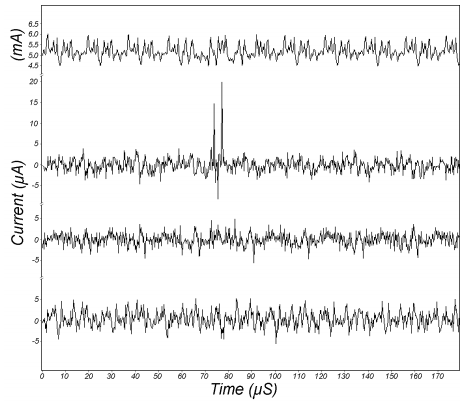
\includegraphics[scale=.7]{dpaTrace}
\caption{DPA traces, one correct and two incorrect, with power reference.}
\label{fig:dpa trace}
\end{figure}


If any bit $b$ of state is correlated with the key, then the difference between when $b=0$ and when $b=1$ will be observable after the noise has been averaged out.  Defenses have proved illusive for differential power analysis, though approaches such as adding random values during computation~\cite{messergesMasking} or ensuring that an equal number of transitions from $0\rightarrow 1$ occur regardless of the key and plaintext~\cite{poppMangardDualRail}.  However, these techniques can be defeated by using either more samples or higher-order differential analysis~\cite{joyeSecondOrderDPA}.

\bibliographystyle{plain}
\bibliography{crypto}
\end{document}

